% Options for packages loaded elsewhere
\PassOptionsToPackage{unicode}{hyperref}
\PassOptionsToPackage{hyphens}{url}
%
\documentclass[
  10pt,
]{article}
\usepackage[]{mathpazo}
\usepackage{amssymb,amsmath}
\usepackage{ifxetex,ifluatex}
\ifnum 0\ifxetex 1\fi\ifluatex 1\fi=0 % if pdftex
  \usepackage[T1]{fontenc}
  \usepackage[utf8]{inputenc}
  \usepackage{textcomp} % provide euro and other symbols
\else % if luatex or xetex
  \usepackage{unicode-math}
  \defaultfontfeatures{Scale=MatchLowercase}
  \defaultfontfeatures[\rmfamily]{Ligatures=TeX,Scale=1}
\fi
% Use upquote if available, for straight quotes in verbatim environments
\IfFileExists{upquote.sty}{\usepackage{upquote}}{}
\IfFileExists{microtype.sty}{% use microtype if available
  \usepackage[]{microtype}
  \UseMicrotypeSet[protrusion]{basicmath} % disable protrusion for tt fonts
}{}
\makeatletter
\@ifundefined{KOMAClassName}{% if non-KOMA class
  \IfFileExists{parskip.sty}{%
    \usepackage{parskip}
  }{% else
    \setlength{\parindent}{0pt}
    \setlength{\parskip}{6pt plus 2pt minus 1pt}}
}{% if KOMA class
  \KOMAoptions{parskip=half}}
\makeatother
\usepackage{xcolor}
\IfFileExists{xurl.sty}{\usepackage{xurl}}{} % add URL line breaks if available
\IfFileExists{bookmark.sty}{\usepackage{bookmark}}{\usepackage{hyperref}}
\hypersetup{
  pdftitle={Lurking in the shadows: The impact of emissions target setting on carbon pricing and enviromental efficiency.},
  pdfauthor={Barry Quinn (Queen's Management School); Ronan Gallagher (Edinburgh Business School); Timo Kuosmanen (Aalto Business School)},
  pdfkeywords={Marginal abatement costs, Enviromental efficiency, Stochastic nonparametric envelopment of data (StoNED), Carbon emissions target setting, Kyoto Protocol, Development economics},
  hidelinks,
  pdfcreator={LaTeX via pandoc}}
\urlstyle{same} % disable monospaced font for URLs
\usepackage[margin=1in]{geometry}
\usepackage{graphicx,grffile}
\makeatletter
\def\maxwidth{\ifdim\Gin@nat@width>\linewidth\linewidth\else\Gin@nat@width\fi}
\def\maxheight{\ifdim\Gin@nat@height>\textheight\textheight\else\Gin@nat@height\fi}
\makeatother
% Scale images if necessary, so that they will not overflow the page
% margins by default, and it is still possible to overwrite the defaults
% using explicit options in \includegraphics[width, height, ...]{}
\setkeys{Gin}{width=\maxwidth,height=\maxheight,keepaspectratio}
% Set default figure placement to htbp
\makeatletter
\def\fps@figure{htbp}
\makeatother
\setlength{\emergencystretch}{3em} % prevent overfull lines
\providecommand{\tightlist}{%
  \setlength{\itemsep}{0pt}\setlength{\parskip}{0pt}}
\setcounter{secnumdepth}{-\maxdimen} % remove section numbering
\usepackage{float}
\usepackage{booktabs}
\usepackage{longtable}
\usepackage{array}
\usepackage{multirow}
\usepackage{wrapfig}
\usepackage{colortbl}
\usepackage{pdflscape}
\usepackage{tabu}
\usepackage{threeparttable}
\usepackage{threeparttablex}
\usepackage[normalem]{ulem}
\usepackage{makecell}
\usepackage{xcolor}

\title{\emph{Lurking in the shadows:} The impact of emissions target setting on
carbon pricing and enviromental efficiency.}
\author{Barry Quinn (Queen's Management School) \and Ronan Gallagher (Edinburgh Business School) \and Timo Kuosmanen (Aalto Business School)}
\date{June 08, 2021}

\begin{document}
\maketitle
\begin{abstract}
This paper interrogates the impact of the Kyoto Protocol target setting
regime on carbon \emph{shadow} pricing and environmental efficiency. We
extract shadow price estimates and efficiency scores from a
comprehensive dataset of 125 countries over the four years period using
the unified StoNED framework. We exploit recent work, which uses the
\emph{least-cost alternative} procedure to estimate CO\textsubscript{2}
marginal abatement costs from initial model estimation. Results reveal
abatement costs are significantly higher for target setting countries,
increase over the sample period, and are an order of magnitude greater
than the prevailing emissions pricing mechanisms. Given the number on
developing countries in our sample, this findings highlights a shadow
price inequality gap at that time. Typically, environmental inefficiency
scores are higher in countries with higher trade to GDP ratios, higher
urban density, and explicit C0\textsubscript{2} emission targets set
under the Kyoto Protocol. Our findings provide insights into the
consequences of policies to curb unwanted byproducts in a regulated
system and reveal \emph{future price} consequences of the regulation
used to mitigate undesirable outputs.
\end{abstract}

\hypertarget{introduction}{%
\section{Introduction}\label{introduction}}

Target setting stringency in climate policy has attracted considerable
debate since the Kyoto Protocol (hereafter KP) (for example, see
Angelis, Di Giacomo, and Vannoni 2019). The impact of climate change and
the production of greenhouse gas (GHG) emissions are existential
challenges of the 21\textsuperscript{st} century. The World Health
Organisation estimates a health risk associated with climate change of
250,000 additional deaths per year between 2030 and 2050, assuming the
status quo of current abatement practices and global economic
growth\footnote{\url{https://www.who.int/news-room/fact-sheets/detail/climate-change-and-health}}.

Färe and Primont (2012) describes shadow prices as `virtual' or
unforeseen costs to a firm's management. A shadow price obtained from an
economic model is the implicit value of \emph{untradeable} outputs such
as pollutants or undesirable by-products (Lee and Zhang 2012).
Technically, they value the marginal product faced by the decision-maker
based on the optimal choice of outputs and inputs, which maximises
utility (Murray 1995). Under the assumption of rationality, shadow
prices reveal the underlying opportunity costs hidden from the
researcher (Kuosmanen, Cherchye, and Sipiläinen 2006). Importantly, this
opportunity cost (economic price) definition can also take the form of
marginal substitution (transformation) rates between inputs
(outputs).{]}. Luhmann, Balk, and Dembowski (2020) argue that shadow
pricing is as crucial as emission pricing (for example, emissions
trading schemes) for appropriate carbon price discovery. They argue
shadow pricing can also be called ``future pricing''. The word
``shadow'' highlights that, for financiers to assess a project's actual
economic value, fuel is priced higher than current levels. The rationale
being, even if there is no carbon emissions pricing, carbon prices are
taken into account, factoring in \emph{future} value ignored by markets.
Shadow prices have a long history of revealing the cost of reducing
undesirable outputs\footnote{Shadow prices assess the costs of producing
  some by-product, or more technically, an undesirable output. They are
  helpful for regulatory and supervision analysis where quality control
  of by-products plays an integral part in the sustainable growth of the
  regulated system. Shadow price usage is dependent on the observability
  of a market price for the undesirable output. When we observe output
  prices, then shadow pricing models can identify the appropriate output
  mix for revenue maximisation. More commonly, shadow price calculations
  numerate the price of an undesirable output in units of foregone
  desirable output.} in terms of reducing the production of desirable
outputs (See Zhou, Zhou, and Fan (2014) for recent literature on shadow
price estimation). Framed in this way, the shadow price of air pollution
emissions is equivalent to a marginal abatement cost and provides
valuable guidance to emission reduction policies.

Lee and Wang (2019) critique the body of work on marginal abatement
costs of CO\textsubscript{2} at the country level. They show that
empirical studies use frontier efficiency methods to estimate shadow
prices (for country and region level analysis see (Cheng et al. 2019;
Du, Hanley, and Wei 2015; Choi, Zhang, and Zhou 2012; Maradan,
Vassiliev, and Others 2005)) where CO\textsubscript{2} pollutants as
treated as undesirable outputs. We argue that these studies
systematically over-estimate the marginal abatement cost by ignoring
actual performance levels, noise, and the ability to abate via
increasing input uses. For instance, an increase in capital investments
into cleaner technology could be an alternative use of inputs. Kuosmanen
and Zhou (2018) show that marginal abatement costs are routinely
overestimated compared to the market prices of CO\textsubscript{2}. They
develop a methodology to counteract this systematic bias, which we
follow in our analysis.

This paper aims to add to this debate by investigating the impact of KP
target setting on carbon pricing and environmental efficiency.
Specifically, we exploit state-of-the-art frontier methods, namely
\textbf{Sto}chastic \textbf{N}onparametric \textbf{e}nvelopment of
\textbf{D}ata (StoNeD), to produce consistent environmental efficiency
and marginal abatement estimates. We further decompose the target
setting effects using a novel statistical procedure introduced in
Gallagher and Quinn (2019). We estimate marginal abatement costs using
efficient frontier shadow prices\footnote{The terms ``opportunity cost''
  and ``shadow price'' are used interchangeably in the efficiency
  literature.}

Our results provide a consistent economic cost of the KP. Taking
advantage of the explicit target-setting regime from 2008 to 2012, we
estimate the marginal abatement cost of CO\textsubscript{2} emissions.
Unlike previous shadow price estimates of CO\textsubscript{2} emissions
calculated ignoring country-level inefficiencies\footnote{Technically,
  abatement cost estimates assume the entity under investigation is on
  the efficient frontier.}, our model uses a quantile approach to
incorporate additional information on the relative inefficiency of each
country. The analysis results in shadow prices measured as the cost of
abatement in constant international dollar terms.

To disentangle abatement cost differences, we apply a trigonometric
procedure proposed in Gallagher and Quinn (2019). This innovative test
reveals that specific target setting countries typical experienced a
higher marginal abatement cost than their non-target setting
counterparts, the estimated difference being economically and
statistically significant. Our findings suggest an unintended
consequence of climate policy target setting. Our paper is a direct
extension of Kuosmanen, Zhou, and Dai (2020) in two ways; the sample
includes a large number of developing countries (non-annex countries)
and provides explicit evidence of a shadow price inequality gap between
\emph{rich and poor} countries. The proposed market mechanism for
trading emissions failed to eliminate this shadow price gap.

In the next section, we will outline the sample design and define the
variables used. Section 2 briefly outlines the innovative model used to
estimate CO\textsubscript{2} emission production. Section 3 presents the
results and some brief discussion.

\hypertarget{literature-review}{%
\section{Literature Review}\label{literature-review}}

The academic inquiry into the effective control of climate change has a
rich 40-year history. Historically, holistic models seek to understand
how human development, societal choices, and the natural world integrate
and influence each other. At their simplistic level, they can provide an
estimate of the social cost of carbon pollutants. This top-down approach
to the economics of climate change has been at the forefront of the
discipline (Vale 2016). Such a global approach may be dating in the face
of stalled international coordination to climate change policy.

In the run-up to the end of the first commitment period of the KP, there
were political moves to create second commitment period targets. The
Doha amendment in 2012 extended the scope of the protocol targets to
cover the period until 2020. The Doha Amendment was a bridge arrangement
up to 2020 until a new global agreement, negotiated in the \emph{Paris
Agreement}, comes into force. There are critical weaknesses to the
top-down methodology of the Paris agreement. Critics cite lacking
explicit targets, weak legal impunity for emissions targets, and a more
explicit international focus as a critical weakness to country
policymakers taking direct ownership of their emissions targets.

As global cooperation seems less attainable in the last decade,
attention in the policy debate has shifted towards a bottom-up strategy
to mitigation solutions. Vale (2016) argues that the lack of collective
political will, in turn, has seen a shift in the scope of the academic
literature. The recent focus on the economics of catastrophic risk
insurance, trade and climate, and climate change adaptation represents a
shift towards a more realistic investigation of climate policy in an age
where the ideal scenario of globally coordinated climate action seems
illusory.

\hypertarget{cost-of-kp-literature}{%
\subsection{Cost of KP literature}\label{cost-of-kp-literature}}

Zhang and Folmer (1998) document and critique the myriad of marginal
abatement cost models. They consider both bottom-up technology-based
models and top-down macroeconomic models. They conclude, a combination
of these models best assesses the overall consequences of controlling
CO\textsubscript{2} emissions. Nordhaus and Boyer (1999) use a
scenario-based approach to analyze the economics of various trading
emission schemes (ETS) for Annex I countries for the KP. They find costs
of the ETS's are seven times greater than the benefits, two/thirds of
the net global cost of \$716 billion, are borne by the US\footnote{Brechin
  (2003) uses various public opinion polls to revisits the questions of
  international public concern for global warming. They find, while the
  perception has been a slight improvement in the public's understanding
  regarding the anthropogenic causes of global warming, the data reveals
  the public remains largely uninformed. They note that President Bush's
  withdrawal of the KP in 1991 was supported mainly by the US public
  while citizens of several European countries voiced considerable
  outrage about the decision.} and conclude that the proposed schemes
are highly cost-ineffective\footnote{Compared to a *so-called" efficient
  abatement strategy for global temperature reduction, the proposed
  strategy was eight times more costly.}.

This early work was suggestive of a broad approach to abatement cost
analytics beyond the consideration of CO\textsubscript{2} pollution.
Reilly et al. (1999) use the Regional Integrated Model of Climate and
Economy (RICE) to show that a multi-gas control strategy could
significantly reduce the costs of fulfilling the KP compared with a
CO\textsubscript{2}-only strategy. Extending the KP to 2100 without more
severe emissions reductions shows little difference between the two
strategies in climate and ecosystem effects. They argue that the global
warming potential of the KP are limited in terms and argue for a more
comprehensive multi-gas approach. Burniaux (2000) extends previous OECD
analysis to emission abatement of methane and nitrous oxide. They
conclude that the economic costs of implementing the targets in the KP
are lower than suggested by previous CO\textsubscript{2}-only results.
In the longer term, most abatement will likely have to come from
CO\textsubscript{2}, and the inclusion of other gases in the analysis
may not substantially alter estimates of economic costs.

In the later years of the KP period, researchers consider a more
statistically sophisticated approach for critiquing the KP. Buonanno,
Carraro, and Galeotti (2003) adapt the RICE integrated assessment model
to account for endogenous technical change\^{} {[}They explore three
formulations; technical change is endogenous and enters the production
function via the domestic stock of knowledge; there is an additional
effect of domestic stock of knowledge on the emission-output ratio; the
output of domestic R\&D spills over the other regions' productivity and
emission-output ratio.{]}. and shows that results are significantly
impacted when modelling R\&D. They find that total costs of compliance
with Kyoto; are higher with induced technical change; are reduced when
trading permits are introduced, and technological spillover reduces the
incentive for R\&D, but overall costs are higher in the presence of
spillovers. McKibbin and Wilcoxen (2004) update their earlier estimates
of the cost of the KP using the
\href{https://unfccc.int/topics/mitigation/workstreams/response-measures/modelling-tools-to-assess-the-impact-of-the-implementation-of-response-measures/response-measures-models-g-cubed}{G-Cubed
model}, taking into account the new sink allowances from recent
negotiations as well as allowing for multiple gases and new land
clearing estimates. They perform a sensitivity analysis of compliance
costs to unexpected changes in future economic conditions. The paper
evaluates the policies under two plausible alternative assumptions about
a single aspect of the future world economy: the rate of productivity
growth in Russia. They find moderate growth in Russia would raise the
cost of the KP by as much as fifty per cent but would have little effect
on the cost of the alternative policy. They conclude that the KP is
inherently unstable because unexpected future events could raise
compliance costs substantially and place enormous pressure on
governments to abrogate the agreement. The alternative policy would be
far more stable because it does not subject future governments to
adverse shocks in compliance costs. Fischer and Morgenstern (2006) find
that estimates of marginal abatement costs for reducing carbon emissions
in the United States by the significant economic-energy models vary by a
factor of five, undermining support for mandatory policies to reduce
greenhouse gas emissions. Their meta-analysis explains which modelling
assumptions are most important for understanding these cost differences
and argues for developing more consistent modelling practices for policy
analysis.

More recent studies focus on a bottom-up approach, showing how a
country's economic characteristics fluctuate with abatement challenges.
Halkos and Tzeremes (2014) applies a probabilistic DEA approach to
estimate conditional and unconditional environmental efficiency of 110
countries in 2007. They find that a country's environmental efficiency
is influenced in a non-linear fashion by both the obliged percentage
levels of emission reductions the duration in which a country has signed
the KP. Cifci and Oliver (2018) use regression techniques to illustrate
the conflicting political strands of the climate change argument. The
results show that the KP reduced Annex I countries GHG emissions by
approximately 1 million metric tons of CO\textsuperscript{2} equivalent
relative to non-Annex I countries. Contrariwise, these countries
experienced an average reduction in GDP per capita growth of 1-2 per
cent relative to non-Annex I countries. Both findings illustrate that
the international climate change agreements are fragile because, at a
national level, political constituencies' value systems may conflict to
reduce greenhouse gas (GHG) emissions to sustainable levels.

\hypertarget{model}{%
\section{Model}\label{model}}

The primary focus of our analysis is shadow prices estimates for
CO\textsubscript{2} emission from fossil fuel. Previous studies have
provided inaccurate measures as a result of several missteps, including:

\begin{itemize}
\tightlist
\item
  only considering downscaling of production and not increasing in input
  use.
\item
  measuring estimates on the frontier, ignoring the actual level of
  performance.
\item
  deterministic estimation, which explicitly ignores the impact of noise
  in the data.
\end{itemize}

These factors combine to overestimate shadow prices, group differences
in shadow prices grossly, and the impact of emissions reduction
targeting. Our study uses convex quantile regression methods to estimate
local approximations of shadow prices calibrated using observed
inefficiencies. Specifically, we exploit the benefits of Kuosmanen and
Johnson (2017) directional distance convex regression and Wang et al.
(2014) quantile formulation to reveal shadow prices at observed
performance levels. Importantly, this approach is robust to the observed
heterogeneity, the choice of direction vector and accommodates
noise-based uncertainty. The following linear programming problem is
solved to estimate the distance function:

\begin{equation}
\begin{split}
& \underset{\alpha,\beta,\gamma,\delta,\epsilon^-,\epsilon^+}{\text{min}}
 (1-\tau) \sum^{T}_{t=1} \sum^{n}_{i=1}\epsilon^-_{it} + \tau \sum^{T}_{t=1}  \sum^{n}_{i=1}\epsilon^+_{it}  \\
&\text{s.t.} \\
&\gamma^{'}_{it}y_{it}=\alpha_{it}+\beta^{'}_{it}x_{it}+\delta^{'}_{it}b_{it} + \omega Z_{it} -\epsilon^-_{it}+\epsilon^+_{it} \; \forall i ,\forall t \\
&\alpha_{it}+\beta^{'}_{it}x_{it}+\delta^{'}_{it}b_{it}-\gamma^{'}_{it}y_{it} \leq \alpha_{hs}+\beta^{'}_{hs}x_{it}+\delta^{'}_{hs}b_{it}-\gamma^{'}_{hs}y_{it} \; \forall i,h ; \forall t,s \\
& \beta^{'}_{it}g^x+\delta^{'}_{it}g^b+\gamma^{'}_{it}g^y=1 \; \forall i,t\\
& \beta_{it} \geq0,\gamma_{it} \geq0,\delta_{it} \geq0 \; \forall i,t \\
& \epsilon^-_{it} \geq0, \epsilon^+_{it} \geq 0 \; \forall i,t
\end{split}
\end{equation}

Equation 1 is a probabilistic distance function, where the two errors
terms (\(\epsilon^-\) and \(\epsilon^+\)) allow for deviations from the
frontier, and \(\tau\) defines the quantile. We estimate the model using
a balanced panel of 105 countries for five years (2008-2012) where the
\(Z\) vector includes, trade to GDP ratio, the percentage of the
population which is urban, a dummy to the indicator if the country is a
target setting, and a set of year dummies. These environmental variable
adjust for observed cross-country and through time fluctuation in the
production technology. The estimated model results in performance
adjusted dual prices \(\gamma^{'}_{it},\beta^{'}_{it} ,\delta^{'}_{it}\)
which serve as inputs for the marginal abatement calculations. An
additional appealing feature of the specification in equation 1 is a
separately estimated intercept for each observation; \(\alpha_{it}\).
These intercept terms are analogous to \emph{random} effects in
multi-level modelling, capturing unobserved time series and
cross-sectional variation.

\hypertarget{marginal-abatement}{%
\subsection{Marginal abatement}\label{marginal-abatement}}

Marginal abatement estimation uses a series of levels to find the local
quantile \(\tau^{*}\) for each observed data point. For example, a set
of ten quantile levels
\(\tau=(0.05,0.15,0.25,0.35,0.45,0.55,0.65,0.75,0.85,0.95)\)\footnote{We
  use the GAMS software and the CPLEX solver to find an optimal solution
  to equation 1}. In general, the number of quantiles is not fixed but
should depend on sample size and signal to noise ratio.

Kuosmanen and Zhou (2018) note that in the traditional approach to
shadow pricing using frontier estimation, marginal abatement costs and
shadow prices are interchangeable terms. This feature is because
previous approaches only use bad output shadow prices measured in
forgone \emph{good} output units. They expand the marginal abatement
cost definition to include incremental use of inputs by considering an
optimal combination of shadow price definitions:

\begin{enumerate}
\def\labelenumi{\arabic{enumi}.}
\tightlist
\item
  The marginal rate of transformation between \emph{good} and \emph{bad}
  outputs (MRT).\\
\item
  The marginal product of inputs on outputs (MP).
\end{enumerate}

In our study, we similarly calculate marginal abatement costs as:

\begin{enumerate}
\def\labelenumi{\arabic{enumi}.}
\tightlist
\item
  Find the largest expectile (\(\tau^{*}\)) for which the residual
  (\(\epsilon^+ + \epsilon^-\)) is non-negative.
\end{enumerate}

\begin{itemize}
\tightlist
\item
  For most observations, we find the nearest expectile by checking where
  the residual \(\epsilon = (\epsilon^+) - (\epsilon^-)\) changes sign.
  For those observations, we take the weighted average of the shadow
  prices of the nearest executives, weighted by \(\epsilon\). For some
  observations, residuals are positive (or negative) for all executives
  (the best and the worst performers, respectively). For those, we use
  shadow prices of the highest/lowest expectile.
\end{itemize}

\begin{enumerate}
\def\labelenumi{\arabic{enumi}.}
\setcounter{enumi}{1}
\item
  Calculate MRT and MP as the weighted average of quantiles for
  (\(\tau^{*}\))r and (\(\tau^{*+1}\)) weighted by the distance to the
  frontier of the quantiles(i.e.~the absolute value of the residuals).
  Specifically these can be thought of as the sub derivatives with
  respect to the bad outputs from the distance function, where the
  marginal rate of substitution of output \(i\) on bad output \(j\) is
  \(MRT_{\tau}(y_{i},b_{j})=-\frac{\delta \vec{D}_{\tau}/\delta b_{j}}{\delta \vec{D}_{\tau}/\delta y_{i}}\).
  Similarly the MP of input k on bad output j is
  \(MP_{\tau}(x_{k},b_{j})=\frac{\delta \vec{D}_{\tau}/\delta b_{j}}{\delta \vec{D}_{\tau}/\delta x_{k}}\)
\item
  Use the results from step 2, the marginal abatement cost (MAC) for bad
  output \(j\) is define as: \begin{equation}
  MAC(b_{j})=\displaystyle \min_{i,k}\{p_{i}MRT_{\tau}(y_{i},b_{j}), w_{k}MP_{\tau}(x_{k},b_{j})\}
  \end{equation}
\end{enumerate}

In equation 2 \(p_{i}\) is the price of output \(i\) and \(w_{k}\) is
the price of input \(k\). This flexible definition of the MAC provides
multiple opportunities for abatement. Specifically, bad output \(j\) can
be abated by either reducing \emph{good} outputs (i.e., downscaling the
GDP activity) or increasing the input use (for example, investment in
the labour force or capital stock). This approach uses the least-cost
alternative. In the case where the \emph{good} outputs possess a
monetary value, the sub derivatives (dual prices) provide monetary
shadow prices for bad outputs, and the above equation simplifies to:

\begin{equation}
MAC(b_{j})=\displaystyle \min_{i,k}\{MRT_{\tau}(y_{i},b_{j}), MP_{\tau}(x_{k},b_{j})\} 
\end{equation}

In the above calculation, it is essential to ensure that the MRT and MP
enter the model simultaneously, given the scale of the inputs and
outputs entering the model. In our model, as both capital stock and GDP
enter the model in billions of dollars, the MRT and MP are directly
comparably in terms of minimum cost.

\hypertarget{application-of-statistical-test}{%
\subsection{Application of Statistical
Test}\label{application-of-statistical-test}}

Appendix A:1 details the theoretical exposition of shadow price group
difference testing first proposed in Gallagher and Quinn (2019). Suppose
we have two series of the output ratio y2/y1, representing two groups of
firms observed in the same period or the same sample of firms observed
in two different periods. There are several methods for testing whether
the two series are significantly different.

An obvious possibility is to apply a two-sample t-test for testing the
equality of means or the F-test for equal variances. This test requires
either that sample size is sufficiently large for asymptotic inferences
or that the ratio y2/y1 is normally distributed.

There are also several nonparametric alternatives. The (Wilcoxon)
Mann-Whitney U tests whether the medians of two independent
distributions are different. Another possibility is the two-sample
Kolmogorov-Smirnov test. If there is a pair of series(e.g., the same
firms observed in two different periods), then nonparametric rank-order
tests such as Spearman's rho and Kendall's tau can be used to test for
correlation between two series of y2/y1.

\hypertarget{testing-procedure}{%
\subsubsection{Testing procedure}\label{testing-procedure}}

There are three steps to the testing procedure for the difference in the
ratio series y2/y1. The first two steps are preliminary in that they
establish the statistical properties of the series, which informs the
choice of group difference test in the three-step.

\begin{enumerate}
\def\labelenumi{\arabic{enumi}.}
\item
  Test the empirical distribution of the series for normality. Whether
  the series is normally distributed determines whether a parametric or
  nonparametric test is needed. Stephens (1986) recommend the use of a
  normality test introduced by Anderson and Darling (1952) Anderson and
  Darling (1954). This procedure is a rank-sum test for goodness of fit
  based on the empirical distribution and has the advantage of giving
  more weight to the tails of the distribution.
\item
  Test the homogeneity of variance in the two groups. If step 1
  establishes normality, a simple F test of the homogeneity of variance
  can be performed. In the presence of non-normality, we turn to the
  Brown and Forsythe (1974) test, which extended the Levene (1961) ANOVA
  procedure applied to absolute deviations from the corresponding group
  mean. This Brown-Forsythe test transforms the variances into the
  absolute values of their deviations from the median. It uses a ratio
  of this transformed data as test statistics (See O'Brien (1981) for
  full explanation).
\item
  If the equal group variance and the normality assumptions are not
  rejected, then perform a Welch t-test for group mean differences
  (Welch 1947). The Kolmogorov-Smirnov nonparametric test provides a
  more robust statistical inference (Conover 1999). If only the
  normality assumption is rejected, the Wilcoxon Mann Whitney test is
  more appropriate.
\end{enumerate}

\hypertarget{data-and-variables}{%
\section{Data and variables}\label{data-and-variables}}

The KP offers a unique empirical framework to assess the effects of
explicit target setting in climate change policy. The first commitment
period for the KP was 2008 to 2012. Countries defined as developing
(non-annexe 1) were not subject to targets, although most ratified the
Protocol. The US was the only signatory of the Protocol that did not
ratify. This decision was likely the combination, a weak green lobby in
Washington DC(Hovi, Sprinz, and Bang 2012), excessive compliance
costs(Manne and Richels 2004), poor public understanding of climate
change (Brechin 2003), and a strong energy lobby during Bush's
tenure.\footnote{Andorra, Palestine, South Sudan and the Vatican also do
  not follow the Protocol. Canada ratified but withdrew effective in
  December 2012.}. In the run-up to the end of the first commitment
period, there were political moves to create targets for a second
commitment period. Critics argued that the Paris agreement fell well
short of the KP in set explicit targets and punitive penalties.

For these reasons, we focus on emissions data from 2008 to 2012, the
first commitment period. For this period, it is easier to say
definitively who had set targets and who had not. The lines got blurred
post-2012 when a new negotiation phase began. The Protocol set a target
for emissions of a basket of greenhouse gases\footnote{carbon dioxide,
  CO\textsuperscript{2}; methane, CH\textsuperscript{4}; nitrous oxide,
  NO\textsuperscript{2}; sulphur fluoride, SF\textsuperscript{6};
  hydrofluorocarbons, HFCs; and perfluorocarbons; PFCs.} to be reached
by the signatories in the period 2008-2012. This paper extends the work
of Halkos and Tzeremes (2014). To the best of our knowledge, it is the
first study to explicitly provide an economic cost for these emissions
targets\footnote{Halkos and Tzeremes (2014) investigate the overall
  environmental efficiency impact of the KP.}.

We specify a two input-two output frontier efficiency model.
Specifically, we define GDP as a desirable output, CO\textsuperscript{2}
emissions from fuel combustion as an undesirable output, and labour
force numbers and capital stock as inputs. GDP and labour force numbers
are sourced from the World Bank. The capital stock captures both current
and past accumulations of capital investment. Finally, to capture
cross-country and time-varying heterogeneity in CO\textsuperscript{2}
production, we use several environmental \(Z\) variables. Table 1
provides a detailed description of the modelling variables.

\begingroup\fontsize{8}{10}\selectfont

\begin{ThreePartTable}
\begin{TableNotes}
\item \textit{Note: } 
\item A detailed description of the inputs, outputs and enviromental variables which index the production frontier model.  Capital stock and GDP are monetary variables and enter the model in real terms measured at purchasing power parity or constant international dollar billions.
\end{TableNotes}
\begin{longtabu} to \linewidth {>{\raggedright\arraybackslash}p{5em}>{\raggedright\arraybackslash}p{5em}>{\raggedright\arraybackslash}p{30em}>{\raggedright\arraybackslash}p{5em}}
\caption{\label{tab:variables}Description of variables}\\
\toprule
Type & Variable & Detail & Source\\
\midrule
\endfirsthead
\caption[]{Description of variables \textit{(continued)}}\\
\toprule
Type & Variable & Detail & Source\\
\midrule
\endhead

\endfoot
\bottomrule
\insertTableNotes
\endlastfoot
Undesirable Output & \textbf{CO2 emissions from fossil fuel (Millions of metric tonnes)} & Emissions were calculated using IEA energy databases and the default methods and emission factors given in the 2006 GLs for National Greenhouse Gas Inventories. & International Energy Agency\\
Desirable Output & \textbf{GDP, PPP (constant 2017 international \$)} & PPP GDP is gross domestic product converted to international dollars using purchasing power parity rates. An international dollar has the same purchasing power over GDP as the U.S. dollar has in the United States. GDP is the sum of gross value added by all resident producers in the country plus any product taxes and minus any subsidies not included in the value of the products. It is calculated without making deductions for depreciation of fabricated assets or for depletion and degradation of natural resources. Data are in constant 2017 international dollars. & International Comparison Program, World Bank | World Development Indicators database, World Bank | Eurostat-OECD PPP Programme.\\
Input & \textbf{Labor force, total} & Labor force comprises people ages 15 and older who supply labor for the production of goods and services during a specified period. It includes people who are currently employed and people who are unemployed but seeking work as well as first-time job-seekers. Not everyone who works is included, however. Unpaid workers, family workers, and students are often omitted, and some countries do not count members of the armed forces. Labor force size tends to vary during the year as seasonal workers enter and leave. & Derived using data from International Labour Organization, ILOSTAT database. The data retrieved in March 1, 2020.\\
Input & \textbf{Capital Stock, PPP (constant international \$Billions)} & Total capital stock is the sum of government capital stock, private capital stock, and public-private partnerships (PPP) capital stock.  When the PPP capital stock is missing we assume zero. & IMF and World Bank\\
Enviromental Variable & \textbf{Trade (\% of GDP)} & Trade is the sum of exports and imports of goods and services measured as a share of gross domestic product. & World Bank national accounts data, and OECD National Accounts data files.\\
\addlinespace
Enviromental Variable & \textbf{Urban population (\% of total population)} & Urban population refers to people living in urban areas as defined by national statistical offices. The data are collected and smoothed by United Nations Population Division. & United Nations Population Division. World Urbanization Prospects: 2018 Revision.\\
Enviromental Variable & \textbf{Target Setting Indicator} & This variable takes a value of 1 for a country which committed to a hard target of emission reduction during the Kyoto Protocol period and zero otherwise. & author's own calculation\\
Enviromental Variable & \textbf{Year Indicators} & A proxy for unobserved between group temporal variation & author's own calculation\\*
\end{longtabu}
\end{ThreePartTable}
\endgroup{}

We use the International Energy Association (IEA) database\footnote{\url{http://data.iea.org/payment/products/115-co2-emissions-from-fuel-combustion-2018-edition-coming-soon.aspx}}
which provides the most extensive global coverage of CO\textsubscript{2}
emission data. This database estimates CO\textsuperscript{2} from fuel
emission measured in Metric Tonnes for over 140 countries from 1960 to
2016. After removing countries with missing observations, we have a
balanced sample of 525 observations for 2008-2012. Table 2 describes the
countries in the sample in terms of target-setting.

\begin{table}[!h]

\caption{\label{tab:targetSetters}Target Setting Countries}
\centering
\fontsize{8}{10}\selectfont
\begin{tabu} to \linewidth {>{\raggedright\arraybackslash}p{20em}>{\raggedright\arraybackslash}p{20em}}
\toprule
Target Setting Country & Non Target Setting Country\\
\midrule
\textbf{Australia, Austria, Belgium, Bulgaria, Canada, Czech Republic, Denmark, Estonia, Finland, France, Germany, Greece, Hungary, Iceland, Ireland, Italy, Japan, Latvia, Luxembourg, Netherlands, New Zealand, Norway, Poland, Portugal, Romania, Russian Federation, Slovak Republic, Spain, Sweden, Switzerland, United Kingdom} & \textbf{Albania, Algeria, Argentina, Armenia, Azerbaijan, Bahrain, Bangladesh, Belarus, Benin, Bolivia, Botswana, Brazil, Cambodia, Cameroon, Chile, China, Colombia, Congo, Rep., Costa Rica, Croatia, Cyprus, Dominican Republic, Ecuador, Egypt, Arab Rep., El Salvador, Georgia, Ghana, Guatemala, Haiti, Honduras, India, Indonesia, Israel, Jamaica, Jordan, Kazakhstan, Kenya, Korea, Rep., Kuwait, Kyrgyz Republic, Lithuania, Malaysia, Malta, Mexico, Morocco, Mozambique, Namibia, Nepal, Nigeria, Oman, Pakistan, Panama, Paraguay, Peru, Philippines, Qatar, Saudi Arabia, Senegal, Singapore, Slovenia, South Africa, Sri Lanka, Sudan, Thailand, Togo, Tunisia, Ukraine, United Arab Emirates, United States, Uruguay, Uzbekistan, Venezuela, RB, Yemen, Rep., Zambia}\\
\bottomrule
\end{tabu}
\end{table}

Some summary statistics of the model variables are presented in Table 3.
These statistics reveal that significant variation in outputs and inputs
highlights considerable cross-sectional heterogeneity. The variation is
not surprising given the mix of countries outlined in table 2.
Furthermore, notice that some countries have a trade which exceeds GDP
(more than 100\%). This excess is usually a feature of small countries
with high productivity. Due to their small size, instead of being
self-sufficient and producing all the products their population needs,
they specialize in a few highly profitable industries. These industries
may produce more money from exports than the entire domestic economy,
which allows them to purchase imports far above what their domestic
economy could otherwise support. For example, in the sample, three
countries have a Trade to GDP ratio of over 200\%; Luxembourg, Malta and
Singapore.

\newpage

\begingroup\fontsize{10}{12}\selectfont

\begin{ThreePartTable}
\begin{TableNotes}
\item \textit{Note: } 
\item This table provides central tendency and spread statistics for the model variables for the sample period by target setting groups. Variables are presented on the measurement basis with which they enter the model, for example Capital stock enters the model in constant \$Billions.
\end{TableNotes}
\begin{longtabu} to \linewidth {>{\raggedright\arraybackslash}p{10em}>{\centering}X>{\centering}X>{\centering}X>{\centering}X>{\centering}X>{\centering}X>{\centering}X>{\centering}X>{\centering}X>{\centering}X}
\caption{\label{tab:sumstats1}Summary statistics of inputs, outputs and z variables}\\
\toprule
\multicolumn{1}{c}{ } & \multicolumn{2}{c}{Mean} & \multicolumn{2}{c}{StdDev} & \multicolumn{2}{c}{5th\%ile} & \multicolumn{2}{c}{Median} & \multicolumn{2}{c}{95th\%ile} \\
\cmidrule(l{3pt}r{3pt}){2-3} \cmidrule(l{3pt}r{3pt}){4-5} \cmidrule(l{3pt}r{3pt}){6-7} \cmidrule(l{3pt}r{3pt}){8-9} \cmidrule(l{3pt}r{3pt}){10-11}
  & Non Target & Target & Non Target & Target & Non Target & Target & Non Target & Target & Non Target & Target\\
\midrule
C02 emissions (Million Metric Tons) & 272.68 & 232.27 & 1086.07 & 346.03 & 2.24 & 7.72 & 22.30 & 66.70 & 496.12 & 1105.97\\
GDP (Billion PPP \$USD) & 764.05 & 910.94 & 2368.19 & 1159.91 & 16.10 & 33.56 & 113.62 & 362.44 & 2662.15 & 3432.20\\
Labour Force (Millions) & 31.82 & 13.60 & 105.78 & 18.58 & 0.81 & 0.24 & 5.53 & 4.94 & 113.96 & 66.18\\
Capital Stock (Billions PPP \$USD) & 1552.25 & 2133.53 & 5168.49 & 2937.17 & 20.80 & 69.57 & 170.11 & 919.89 & 5832.42 & 7321.33\\
Urban to Total Population (\%) & 60.32 & 75.83 & 21.00 & 11.44 & 24.15 & 54.88 & 59.75 & 77.00 & 94.21 & 93.53\\
\addlinespace
Trade to GDP (\%) & 88.35 & 99.64 & 55.18 & 57.63 & 34.16 & 43.18 & 75.73 & 84.75 & 158.02 & 181.70\\
\bottomrule
\insertTableNotes
\end{longtabu}
\end{ThreePartTable}
\endgroup{}

\hypertarget{results-and-discussion}{%
\section{Results and discussion}\label{results-and-discussion}}

We estimate a stepwise yield curve of probabilistic benchmark
technologies. These technologies extract, at the observed performance
level, country-year marginal abatement costs of CO\textsubscript{2}
emissions. We use the direction vector \(g(x)=\bar{x}, g(y)=0, g(x)=0\)
to estimate the directional distance function model for 10 quantiles
\(\tau=(0.05,0.15,\dots,0.85,0.95)\), which should be sufficient
granularity for a sample size of 525. Finally, we include a noise term
that can capture measurement error in the data.

\begin{ThreePartTable}
\begin{TableNotes}
\item \textit{Note: } 
\item This table presents yearly mean and interquartile estimates of the marginal abatement costs calculated for the full sample and for each group of countries.  The last four columns disaggregates the mean analysis to compare countries which set emission reduction targets against countries which did not.  GDP(y) and capital stock (x1) are deflated to 2011 international dollars, and are considered to have a unit price.  An alternative interpretation is that the the price multipliers (p,w)=1 in the calculations of the marginal rate of transformation of GDP and the marginal product of the capital stock as they represent both quantity and price. The marginal abatement cost is thus calculated as the minimum of the marginal rate of transformation of GDP and the marginal product of capital stock on C0\textasciitilde{}2\textasciitilde{} emissions.  The MAC is measured in USD per metric ton of CO\textasciitilde{}2\textasciitilde{} emission. Labour (x2) is the total labour force in each country (in millions).  The marginal product of labour is the dual without a price multiplier and is measured in millions of labour force per ton of CO2 emission.
\end{TableNotes}
\begin{longtabu} to \linewidth {>{\centering}X>{\centering}X>{\centering}X>{\centering}X>{\centering}X>{\centering}X>{\centering}X}
\caption{\label{tab:SPs2}Marginal abatement costs in 2011 dollars per CO2 tonne}\\
\toprule
\multicolumn{1}{c}{\em{\textbf{}}} & \multicolumn{2}{c}{\em{\textbf{Full Sample}}} & \multicolumn{2}{c}{\em{\textbf{Target Setting Countries}}} & \multicolumn{2}{c}{\em{\textbf{Non Target Setting Countries}}} \\
\cmidrule(l{3pt}r{3pt}){2-3} \cmidrule(l{3pt}r{3pt}){4-5} \cmidrule(l{3pt}r{3pt}){6-7}
\em{\textbf{}} & \em{\textbf{Mean}} & \em{\textbf{Interquartile Range}} & \em{\textbf{Mean}} & \em{\textbf{Interquartile Range}} & \em{\textbf{Mean}} & \em{\textbf{Interquartile Range}}\\
\midrule
2008 & 71.91 & 53.59 & 64.45 & 46.22 & 74.95 & 55.35\\
2009 & 81.18 & 63.47 & 90.09 & 40.74 & 77.64 & 63.37\\
2010 & 87.89 & 72.61 & 95.93 & 53.77 & 84.19 & 75.52\\
2011 & 86.73 & 60.64 & 89.64 & 51.83 & 85.46 & 84.99\\
2012 & 103.31 & 67.47 & 111.07 & 75.47 & 100.23 & 58.25\\
\bottomrule
\insertTableNotes
\end{longtabu}
\end{ThreePartTable}

Table 4 summarises the marginal abatement cost estimates for each year
in our sample period. This table presents the mean and interquartile
range for the entire sample, targeting setting countries and their
non-target setting counterparts. Marginal abatement costs illustrate the
carbon intensity, where countries with larger manufacturing sectors will
have relatively higher MAC estimates. The MAC estimates are similar to
those reported in the literature (Lee and Wang 2019; Böhringer and Vogt
2003; Viguier, Babiker, and Reilly 2003). , and comparatively similar to
the cost of C0\textsubscript{2} capture and storage of coal plants
estimated by Rubin, Davison, and Herzog (2015), who estimates a
mitigation cost (constant 2013 dollar per metric tonne of
CO\textsubscript{2}) for the capture of \emph{46-99 US dollars} and
storage of \emph{53-137 US dollars}.

\hypertarget{carbon-emissions-pricing-comparison}{%
\subsection{Carbon emissions pricing
comparison}\label{carbon-emissions-pricing-comparison}}

There is a common theoretical starting point for \emph{carbon emissions}
pricing and \emph{carbon shadow} pricing, a sufficiently high emissions
price for imposing zero emissions that cause global warming. An
appropriate carbon pricing regime should treat these two options as
mutually reinforcing. Carbon emission pricing being where policymakers
add a carbon component to the current market price of pollutants, Shadow
pricing, which ascertains a \emph{future price} of the actual economic
cost of a climate-relevant project. Both have a real-world impact in
that they drive markets towards factoring in long-term impacts. In
practice, the pricing schemes diverge due to political inconvenience and
inadequate multilateral commitments.

Since the introduction of the KP, emission pricing schemes are political
motivators to state actors, where it is politically inconvenient to
increase such tax in line with climate impacts. While efforts such as
the EU emission trading scheme, introduced in 2008 for major industrial
facilities, have been shown to only cover about 40\% of the European
greenhouse-gas emissions\footnote{\url{https://www.dandc.eu/en/article/why-carbon-emissions-pricing-and-carbon-shadow-pricing-both-make-sense\#}:\textasciitilde:text=Appropriate\%20carbon\%20prices\&text=\%E2\%80\%9CCarbon\%20emissions\%20pricing\%E2\%80\%9D\%20means\%20that,not\%20reflect\%20those\%20impacts\%20yet.}.
In contrast, shadow pricing essentially bypasses national governments,
as it is in commonly used by multilateral development banks. At present,
only projects in emerging and developing countries routinely apply
shadow pricing (Luhmann, Balk, and Dembowski 2020). The approach
essentially adopted here is a social value of carbon (SVC). The Stiglitz
and Stern (2017) commission report established an SVC shadow price range
necessary to achieve the Paris temperature target as
\$40-80/tCO\textsubscript{2} by 2020, and \$50-100/tCO\textsubscript{2}
by 2030.

\begin{figure}[H]
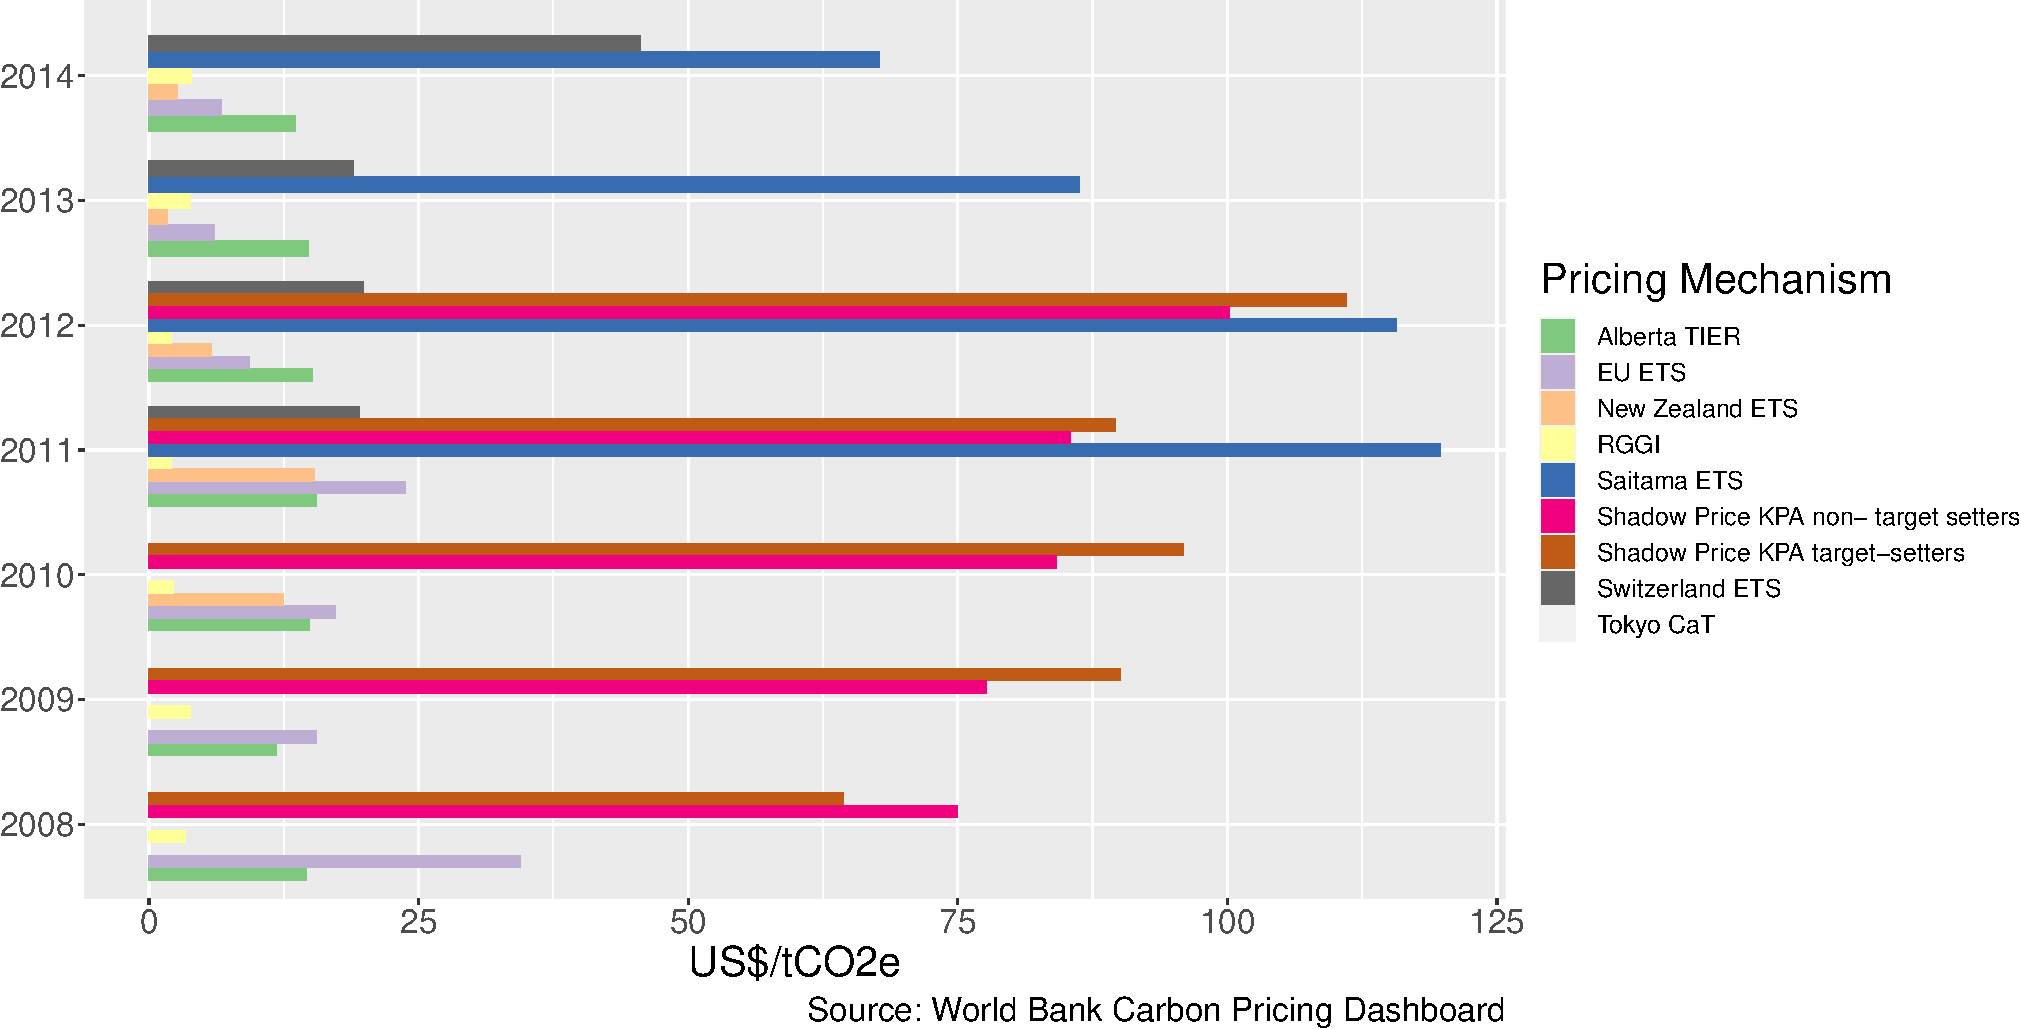
\includegraphics{figures/paper-ETS comparision-1} \caption{ETS pricing mechanism comparison}\label{fig:ETS comparision}
\end{figure}

Figure 1 compares the 2011 nominal Carbon Prices from the EU emission
trading schemes (ETS) to our shadow price mean estimates. Over the four
years of the KP, the shadow price for both groups (target setting and
non-target setting) is a multiple of the prices from the ETS. While our
estimates trend up over the period the ETS prices actually fall.
Interestingly, in the last year the EU-ETS price has increased
dramatically and is beginning to approach our shadow price estimates.

For an emissions trading scheme to work efficiently, allocation of
abatement across countries would require that the marginal abatement
cost is the same in all countries and over time. The results from table
4 suggest this is not the case. The mean MAC is trending up in both
groupings and is typically most significant for target setting
countries. Furthermore, the EU-ETS market, which allows firms from
different countries to buy and sell CO\textsubscript{2} emission
allowances to achieve an efficient allocation of abatement, are not
working to lower the marginal abatement costs of the period. This visual
argument suggests a consistent misallocation of CO\textsubscript{2}
abatement across countries and significant frictions in ETS market price
discovery.

\hypertarget{marginal-effect-of-the-environmental-variable}{%
\subsection{Marginal effect of the environmental
variable}\label{marginal-effect-of-the-environmental-variable}}

Following Gallagher and Quinn (2019), we investigate the marginal effect
of the environmental variables in equation 1 to understand how they
impact inefficiency. Specifically, we consider how inefficiency is
affected by the proportion of trade to GDP, the percentage of the urban
living in a country's population, and whether the country explicitly
sets CO\textsubscript{2} emission targets in the analysis period.

\begin{ThreePartTable}
\begin{TableNotes}
\item \textit{Note: } 
\item This table shows the marginal effects from the z coefficients in equation (1) by exploiting statistical procedure first outlined in Kuosmenan \& Johnson (2015).
\end{TableNotes}
\begin{longtabu} to \linewidth {>{\centering}X>{\centering}X>{\centering}X>{\centering}X>{\centering}X}
\caption{\label{tab:reg}Marginal effect of enviromental variables}\\
\toprule
term & estimate & std.error & statistic & p.value\\
\midrule
TRADEtoGDP & 0.002 & 0.000 & 4.567 & 0.000\\
URBAN & 0.031 & 0.001 & 23.856 & 0.000\\
Setter1 & 0.628 & 0.056 & 11.277 & 0.000\\
Yr2009 & -0.016 & 0.075 & -0.209 & 0.834\\
Yr2010 & -0.013 & 0.075 & -0.169 & 0.866\\
\addlinespace
Yr2011 & -0.014 & 0.075 & -0.191 & 0.849\\
Yr2012 & -0.016 & 0.075 & -0.216 & 0.829\\
\bottomrule
\insertTableNotes
\end{longtabu}
\end{ThreePartTable}

The results from table 5 reveal some interesting features of the
inefficient patterns at the country level. Typically, those with higher
trade to GDP ratios and higher urban populations tend to be less
efficient over the sample. Interestingly, those countries which are
setting targets tend to be more inefficient in the sample period.
Finally, there is an overall reduction in inefficiency over the period
indicated by the year dummies, although this relationship is not
significant in the data.

\hypertarget{application-of-testing}{%
\subsection{Application of testing}\label{application-of-testing}}

Our statistical shadow price difference test is based on the underlying
data for frontier efficiency. Specifically, it is the ratio of the
corresponding bad output to either good output or input that is
represented in a shadow price estimate. For example the ratio of
CO\textsuperscript{2} emissions to GDP could be used to test statistical
differences in the shadow price of the good output calculated as
\(MRT_{\tau}(y_{i},b_{j})=-\frac{\delta \vec{D}_{\tau}/\delta b_{j}}{\delta \vec{D}_{\tau}/\delta y_{i}}\).

\begin{table}[H]

\caption{\label{tab:Test1}Statistical Analysis of Marginal Abatement Cost Differences}
\centering
\begin{threeparttable}
\begin{tabular}[t]{lcccc}
\toprule
\multicolumn{1}{c}{\em{\textbf{}}} & \multicolumn{2}{c}{\em{\textbf{Preliminary}}} & \multicolumn{2}{c}{\em{\textbf{Group Difference }}} \\
\cmidrule(l{3pt}r{3pt}){2-3} \cmidrule(l{3pt}r{3pt}){4-5}
  & Normality Test & Equality of Variance & Rank sum z-test & Equality of distribution D-test\\
\midrule
2008 & 4.25 * * * & 2.83 & 25.8 * * * & 0.64 * * *\\
2009 & 4.3 * * * & 2.92 & 25.51 * * * & 0.62 * * *\\
2010 & 4.18 * * * & 2.29 & 25.58 * * * & 0.64 * * *\\
2011 & 4.2 * * * & 2.64 & 23.97 * * * & 0.62 * * *\\
2012 & 4.08 * * * & 2.95 & 23.09 * * * & 0.62 * * *\\
\bottomrule
\end{tabular}
\begin{tablenotes}
\item \textit{Note: } 
\item This table provides the group difference statistical testing on the ratios of the bad output with either GDP and Capital depending on which corresponding shadow price satisfying MAC equation. Column 1 presents the Anderson Darling test which is the recommended empirical distribution test for normality by Stephens (1986) as it as it gives more weight to the tails of the distribution.  If normality is rejected, we perform heterogeneity of variance tests. The Brown-Forsythe test is presented in column 2 and is robust in the presence of non-normal data. Finally, columns 3 and 4 present the non-parametric group differenc tests.
\end{tablenotes}
\end{threeparttable}
\end{table}

Table 6 shows the results of the testing approach described in test
steps applied each year to the ratio of the variables represented by the
MAC estimates. The first column presents the test results of the
empirical distribution of the ratio and shows that normality is rejected
for all years. This result means we should use a nonparametric group
difference test. Column 2 presents the equality of variance test across
the groups of interest, robust to non-normal distribution. Equality of
variance is not rejected for all years. Columns 3 and 4 of Table 6
provide a statistical analysis of the observed mean differences in
shadow prices presented in table 4. In column 3, the Wilcoxon Mann
Whitney test provides robust inference when we cannot reject the
hypothesis of equality of variance in groups assessed in column 2. The
Kolmogorov Smirnov test provides robust inference if the equality of
variance hypothesis is rejected. Given the results of column 2, column 3
results suggest a statistically significant difference in the shadow
prices of the two cohorts. This finding provides some meaningful
evidence that target setting countries consistently experienced
increased abatement costs over the Kyoto protocol period. \newpage

\hypertarget{concluding-remarks}{%
\section{Concluding Remarks}\label{concluding-remarks}}

This study provides substantial evidence to the ongoing debate on target
setting implications in climate policy. We use a unifying frontier
efficiency approach that reveals some essential and economically
meaningful CO\textsubscript{2} emissions target setting implications.
The study exploits the explicit target setting period of the Kyoto
Protocol to reveal unintended consequences in terms of increased
inefficiencies and marginal abatement costs.

The results reveal important implications for emissions trading schemes.
For an emissions trading scheme to work efficiently, allocation of
abatement across countries would require that the marginal abatement
cost is the same in all countries and over time. Table 4 shows a
substantive difference across the groups, with the mean MAC increasing
over time and typically more significant for target setting countries.

Furthermore, the various regional ETS carbon price discovery mechanisms,
which allow firms from different countries to buy and sell
CO\textsubscript{2} emission allowances to achieve an efficient
allocation of abatement, are not working to lower the marginal abatement
costs of the period. Our chronological ordering analysis suggests a
consistent inefficient allocation of CO\textsubscript{2} abatement
across countries and significant frictions in ETS market price
discovery.

Finally, marginal effects estimate of the environmental variables
suggests that setting the explicit emissions targets result, having
higher trade and more urbanisation typically induces more environmental
inefficiency.

Taking together, our results add value to the regulatory economic
analysis toolbox, by providing a coherent means to investigate
statistically meaningful differences in regulating climate change and
the price discovery markets for pollutants.

\newpage

\hypertarget{appendix}{%
\section{Appendix}\label{appendix}}

\hypertarget{a.1-shadow-price-group-difference-testing}{%
\subsection{A.1: Shadow price group difference
testing}\label{a.1-shadow-price-group-difference-testing}}

We illustrate our test using a cost function but argue it can be
generalised to any production technology specification. Färe and Primont
(2012) prove, using duality theory, that production technologies are
validly represented by either a cost function, the conventional
production function, or a distance function. The cost function is
defined as: \begin{equation}
C(x,y)=\text{min} \{wx:\text{input x can produce output y}\}
(\#eq:CostFn)
\end{equation} where \(x\) is the input vector, \(w\) is the vector of
input prices, and \(y\) is the vector of \(M\) outputs. To estimate the
cost function from data, we assume a cost frontier model:
\begin{equation}
X=C(x,y) + \epsilon
(\#eq:CostFront)
\end{equation} where \(X\) is the observed cost and \(\epsilon\) is a
random disturbance term. The partial derivative of \(C\) with respect to
output \(m\) is referred to as the shadow price of output \(m\) (in
other words, the marginal cost). The vector of all \(M\) shadow prices
is called the gradient vector and is denoted by \(VC\). Figure 2
illustrates the output isoquant in the case of two firms, where the
gradient vector \(VC\) includes two shadow prices illustrated by the
dashed lines. The shadow prices define the slope of the tangent line on
the output frontier.

\begin{figure}[H]
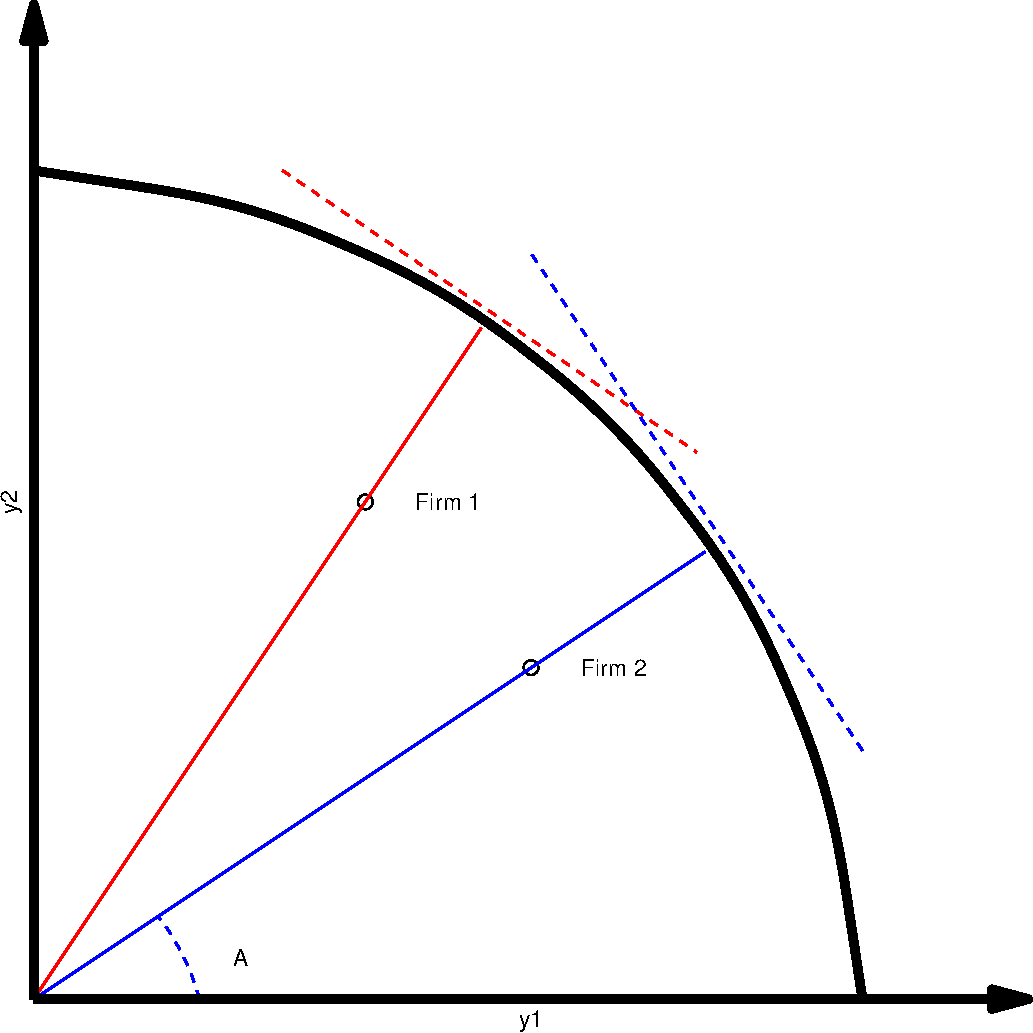
\includegraphics{figures/paper-isoquant-1} \caption{ Two output isoquant}\label{fig:isoquant}
\end{figure}

\begin{footnotesize} 
The figure represents a two output production model, where the black arc line is the best practice output frontier. Firm one and Firm two are operating below the frontier and are inefficient. These firms can improve their production efficiency (move towards the output frontier) by simultaneously producing more y2 and y1 for a given level of inputs (costs). Efficiency for each firm is the length of the dashed lines from the origin, the radial distance.  The dashed tangents on the output frontier represent the shadow prices for the firms.
\end{footnotesize}

From figure 2, it is easy to see that the shadow prices depend on both
the curvature of the output isoquant and the output mix, which the ratio
y2/y1 can measure. Note that tan A = y2/y1, where A is the angle
indicated in figure 2. Note further that the shadow prices depend on
this angle (the polar coordinates), \textbf{not} the distance to the
frontier. Proportional scaling of all outputs by some arbitrary constant
along the dashed rays from the origin does not affect the shadow prices.

What if we have empirically observed a change in the shadow prices (via
some regulatory or supervisory shock), and our objective is to test
whether this change is statistically significant? If the output isoquant
is held constant, the shadow prices can only change due to a change in
the output mix y2/y1. Therefore, we can test if there is a significant
change in the output mix. Note that the ratio y2/y1 is entirely
independent of the estimation of the frontier. Therefore, the test is
immune to possible serial correlation in the finite sample estimates of
the shadow prices. Some standard approaches to testing the significance
of the changes in the distribution of y2/y1 are reviewed in the next
section\footnote{For completeness, it is worth noting that if the output
  isoquant is linear (outputs are perfect substitutes in production),
  then the shadow prices do not change even if the output mix changes.
  We could test if the curvature of the output set is significant (i.e.,
  if there are significant economies of scope) by comparing the linear
  and convex regression (see Meyer (2003), for details), but this is not
  our primary objective. Instead, we are interested in the effect of a
  change in the regulatory and supervisory environment on shadow prices.
  This effect can only occur through the change in the output mix}.

Regulation can influence the output allocation, but not the economies of
scope or the shape of the production possibility set. Zhou, Zhou, and
Fan (2014) argues that a genuine objective of a production unit in the
presence of the introduction of a regulatory abatement target is to
reduce their undesirable output to the target level. If there is an
external abatement target, the producer primarily focuses on achieving
that target emissions level. After attaining this target, the economic
objective of the producer is to maximise the production of the desired
output to maximise profit. Thus, this external regulatory shock changes
the output allocation mix of desirable output to undesirable output but
not the shape of the production possibility set.

As a practical example, consider a regulatory shock that imposes a new
supervisory framework on a regulated system. In the efficiency
literature, regulatory externalities impose technological shifts to the
best-practice frontier technology (the solid line in figure 2). If Hicks
neutrality can be assumed, the effect on the frontier is a parallel
shift where the shape of the production possibility set remains
unchanged.

\newpage

\hypertarget{references}{%
\section*{References}\label{references}}
\addcontentsline{toc}{section}{References}

\hypertarget{refs}{}
\leavevmode\hypertarget{ref-Anderson1952}{}%
Anderson, T W, and D A Darling. 1952. ``Asymptotic Theory of Certain
`Goodness of Fit' Criteria Based on Stochastic Processes.'' \emph{Ann.
Math. Stat.} 23 (2): 193--212.

\leavevmode\hypertarget{ref-Anderson1954}{}%
---------. 1954. ``A Test of Goodness of Fit.'' \emph{J. Am. Stat.
Assoc.} 49 (268): 765--69.

\leavevmode\hypertarget{ref-De_Angelis2019}{}%
Angelis, Enrico Maria de, Marina Di Giacomo, and Davide Vannoni. 2019.
``Climate Change and Economic Growth: The Role of Environmental Policy
Stringency.'' \emph{Sustain. Sci. Pract. Policy} 11 (8): 2273.

\leavevmode\hypertarget{ref-Bohringer2003}{}%
Böhringer, Christoph, and Carsten Vogt. 2003. ``Economic and
Environmental Impacts of the Kyoto Protocol.'' \emph{Canadian Journal of
Economics/Revue Canadienne d'économique} 36 (2): 475--96.

\leavevmode\hypertarget{ref-Brechin2003}{}%
Brechin, Steven R. 2003. ``Comparative Public Opinion and Knowledge on
Global Climatic Change and the Kyoto Protocol: The US Versus the
World?'' \emph{Int. J. Sociol. Soc. Policy} 23 (10): 106--34.

\leavevmode\hypertarget{ref-Brown1974}{}%
Brown, Morton B, and Alan B Forsythe. 1974. ``Robust Tests for the
Equality of Variances.'' \emph{J. Am. Stat. Assoc.} 69 (346): 364--67.

\leavevmode\hypertarget{ref-Buonanno2003}{}%
Buonanno, Paolo, Carlo Carraro, and Marzio Galeotti. 2003. ``Endogenous
Induced Technical Change and the Costs of Kyoto.'' \emph{Res. Energy
Econ.} 25 (1): 11--34.

\leavevmode\hypertarget{ref-Burniaux2000}{}%
Burniaux, Jean-Marc. 2000. ``A Multi-Gas Assessment of the Kyoto
Protocol.'' \emph{OECD Economics Department Working Papers No. 270}.

\leavevmode\hypertarget{ref-Cheng2019}{}%
Cheng, Yu, Kangjuan Lv, Jian Wang, and Hao Xu. 2019. ``Energy
Efficiency, Carbon Dioxide Emission Efficiency, and Related Abatement
Costs in Regional China: A Synthesis of Input--Output Analysis and
DEA.'' \emph{Energy Efficiency}.

\leavevmode\hypertarget{ref-Choi2012}{}%
Choi, Yongrok, Ning Zhang, and P Zhou. 2012. ``Efficiency and Abatement
Costs of Energy-Related CO2 Emissions in China: A Slacks-Based
Efficiency Measure.'' \emph{Appl. Energy} 98 (October): 198--208.

\leavevmode\hypertarget{ref-Cifci2018}{}%
Cifci, Eren, and Matthew E Oliver. 2018. ``Reassessing the Links Between
GHG Emissions, Economic Growth, and the UNFCCC: A
Difference-in-Differences Approach.'' \emph{Sustain. Sci. Pract. Policy}
10 (2): 334.

\leavevmode\hypertarget{ref-Conover1999}{}%
Conover, W J. 1999. \emph{Practical Nonparametric Statistics}. 3
edition. Wiley.

\leavevmode\hypertarget{ref-Du2015}{}%
Du, Limin, Aoife Hanley, and Chu Wei. 2015. ``Marginal Abatement Costs
of Carbon Dioxide Emissions in China: A Parametric Analysis.''
\emph{Environmental and Resource Economics}.

\leavevmode\hypertarget{ref-Fare2012}{}%
Färe, Rolf, and Daniel Primont. 2012. \emph{Multi-Output Production and
Duality: Theory and Applications}. Springer Netherlands.

\leavevmode\hypertarget{ref-Fischer2006}{}%
Fischer, Carolyn, and Richard D Morgenstern. 2006. ``Carbon Abatement
Costs: Why the Wide Range of Estimates?'' \emph{Energy J.} 27 (2):
73--86.

\leavevmode\hypertarget{ref-Gallagher2019}{}%
Gallagher, Ronan, and Barry Quinn. 2019. ``Regulatory Own Goals: The
Unintended Consequences of Economic Regulation in Professional
Football.'' \emph{European Sport Management Quarterly}, April, 1--20.

\leavevmode\hypertarget{ref-Halkos2014}{}%
Halkos, George E, and Nickolaos G Tzeremes. 2014. ``Measuring the Effect
of Kyoto Protocol Agreement on Countries' Environmental Efficiency in
CO2 Emissions: An Application of Conditional Full Frontiers.'' \emph{J
Prod Anal} 41 (3): 367--82.

\leavevmode\hypertarget{ref-Hovi2012}{}%
Hovi, Jon, Detlef F Sprinz, and Guri Bang. 2012. ``Why the United States
Did Not Become a Party to the Kyoto Protocol: German, Norwegian, and US
Perspectives.'' \emph{European Journal of International Relations} 18
(1): 129--50.

\leavevmode\hypertarget{ref-Kuosmanen2006}{}%
Kuosmanen, Timo, Laurens Cherchye, and Timo Sipiläinen. 2006. ``The Law
of One Price in Data Envelopment Analysis: Restricting Weight
Flexibility Across Firms.'' \emph{Eur. J. Oper. Res.} 170 (3): 735--57.

\leavevmode\hypertarget{ref-Kuosmanen2017}{}%
Kuosmanen, Timo, and Andrew Johnson. 2017. ``Modeling Joint Production
of Multiple Outputs in StoNED: Directional Distance Function Approach.''
\emph{Eur. J. Oper. Res.} 262 (2): 792--801.

\leavevmode\hypertarget{ref-Kuosmanen2018b}{}%
Kuosmanen, Timo, and Xun Zhou. 2018. ``Shadow Prices and Marginal
Abatement Costs: Convex Quantile Regression Approach,'' November.

\leavevmode\hypertarget{ref-Kuosmanen2020}{}%
Kuosmanen, Timo, Xun Zhou, and Sheng Dai. 2020. ``How Much Climate
Policy Has Cost for OECD Countries?'' \emph{World Dev.} 125 (January):
104681.

\leavevmode\hypertarget{ref-Lee2019}{}%
Lee, Chia-Yen, and Ke Wang. 2019. ``Nash Marginal Abatement Cost
Estimation of Air Pollutant Emissions Using the Stochastic
Semi-Nonparametric Frontier.'' \emph{Eur. J. Oper. Res.} 273 (1):
390--400.

\leavevmode\hypertarget{ref-Lee2012}{}%
Lee, Myunghun, and Ning Zhang. 2012. ``Technical Efficiency, Shadow
Price of Carbon Dioxide Emissions, and Substitutability for Energy in
the Chinese Manufacturing Industries.'' \emph{Energy Econ.} 34 (5):
1492--7.

\leavevmode\hypertarget{ref-Levene1961}{}%
Levene, Howard. 1961. ``Robust Tests for Equality of Variances.''
\emph{Contributions to Probability and Statistics. Essays in Honor of
Harold Hotelling}, 279--92.

\leavevmode\hypertarget{ref-Luhmann2020}{}%
Luhmann, Hans-Jochen, Sabine Balk, and Hans Dembowski. 2020. ``Why
Carbon Emissions Pricing and Carbon Shadow Pricing Both Make Sense.''
\emph{Development and Cooperation}.

\leavevmode\hypertarget{ref-Manne2004}{}%
Manne, Alan, and Richard Richels. 2004. ``US Rejection of the Kyoto
Protocol: The Impact on Compliance Costs and CO2 Emissions.''
\emph{Energy Policy} 32 (4): 447--54.

\leavevmode\hypertarget{ref-Maradan2005}{}%
Maradan, David, Anatoli Vassiliev, and Others. 2005. ``Marginal Costs of
Carbon Dioxide Abatement: Empirical Evidence from Cross-Country
Analysis.'' \emph{Revue Suisse d Economie et de Statistique} 141 (3):
377.

\leavevmode\hypertarget{ref-McKibbin2004}{}%
McKibbin, Warwick J, and Peter J Wilcoxen. 2004. ``Estimates of the
Costs of Kyoto: Marrakesh Versus the McKibbin--Wilcoxen Blueprint.''
\emph{Energy Policy} 32 (4): 467--79.

\leavevmode\hypertarget{ref-Meyer2003}{}%
Meyer, Mary C. 2003. ``A Test for Linear Versus Convex Regression
Function Using Shape‐restricted Regression.'' \emph{Biometrika} 90 (1):
223--32.

\leavevmode\hypertarget{ref-Murray1995}{}%
Murray, Brian C. 1995. ``Measuring Oligopsony Power with Shadow Prices:
U.S. Markets for Pulpwood and Sawlogs.'' \emph{Rev. Econ. Stat.} 77 (3):
486--98.

\leavevmode\hypertarget{ref-Nordhaus1999}{}%
Nordhaus, William D, and Joseph G Boyer. 1999. ``Requiem for Kyoto: An
Economic Analysis of the Kyoto Protocol.'' \emph{Energy J.} 20: 93--130.

\leavevmode\hypertarget{ref-OBrien1981}{}%
O'Brien, Ralph G. 1981. ``A Simple Test for Variance Effects in
Experimental Designs.'' \emph{Psychol. Bull.} 89 (3): 570--74.

\leavevmode\hypertarget{ref-Reilly1999}{}%
Reilly, J, R Prinn, J Harnisch, J Fitzmaurice, H Jacoby, D Kicklighter,
J Melillo, P Stone, A Sokolov, and C Wang. 1999. ``Multi-Gas Assessment
of the Kyoto Protocol.'' \emph{Nature} 401 (6753): 549--55.

\leavevmode\hypertarget{ref-Rubin2015}{}%
Rubin, Edward S, John E Davison, and Howard J Herzog. 2015. ``The Cost
of CO2 Capture and Storage.'' \emph{Int. J. Greenhouse Gas Control} 40
(September): 378--400.

\leavevmode\hypertarget{ref-Stephens1986}{}%
Stephens, Michael A. 1986. ``Tests Based on EDF Statistics.'' In
\emph{Goodness-of-Fit-Techniques}, 97--194. Routledge.

\leavevmode\hypertarget{ref-CPLC2017}{}%
Stiglitz, Joseph E., and Nicholas Stern. 2017. ``Report of the
High-Level Commission on Carbon Prices.'' \emph{Carbon Pricing
Leadership Coalition}. Routledge.
\url{https://static1.squarespace.com/static/54ff9c5ce4b0a53decccfb4c/t/59b7f2409f8dce5316811916/1505227332748/CarbonPricing_FullReport.pdf}.

\leavevmode\hypertarget{ref-Vale2016}{}%
Vale, Petterson Molina. 2016. ``The Changing Climate of Climate Change
Economics.'' \emph{Ecol. Econ.} 121 (January): 12--19.

\leavevmode\hypertarget{ref-Viguier2003}{}%
Viguier, Laurent L, Mustafa H Babiker, and John M Reilly. 2003. ``The
Costs of the Kyoto Protocol in the European Union.'' \emph{Energy
Policy} 31 (5): 459--81.

\leavevmode\hypertarget{ref-Wang2014}{}%
Wang, Yongqiao, Shouyang Wang, Chuangyin Dang, and Wenxiu Ge. 2014.
``Nonparametric Quantile Frontier Estimation Under Shape Restriction.''
\emph{Eur. J. Oper. Res.} 232 (3): 671--78.

\leavevmode\hypertarget{ref-Welch1947}{}%
Welch, B L. 1947. ``The Generalisation of Student's Problems When
Several Different Population Variances Are Involved.'' \emph{Biometrika}
34 (1-2): 28--35.

\leavevmode\hypertarget{ref-Zhang1998}{}%
Zhang, Zhongxiang, and Henk Folmer. 1998. ``Economic Modelling
Approaches to Cost Estimates for the Control of Carbon Dioxide
Emissions.'' \emph{Energy Econ.} 20 (1): 101--20.

\leavevmode\hypertarget{ref-Zhou2014}{}%
Zhou, P, X Zhou, and L W Fan. 2014. ``On Estimating Shadow Prices of
Undesirable Outputs with Efficiency Models: A Literature Review.''
\emph{Appl. Energy} 130 (October): 799--806.

\end{document}
